\subsection{Escenario Experimental B} \label{sec:EscenarioExperimentalB}

El segundo escenario, busca el evaluar la capacidad de la implementación en donde ya existen componentes en ejecución, al igual que el manejo de múltiples aplicaciones. Para esto, se definieron dos aplicaciones, como se observa en la figura \ref{fig:ExpB}, 

\begin{figure}[H]
    \centering
    \caption{\\Aplicaciones definidas para el desarrollo del escenario experimental B}
    \label{fig:ExpB}
    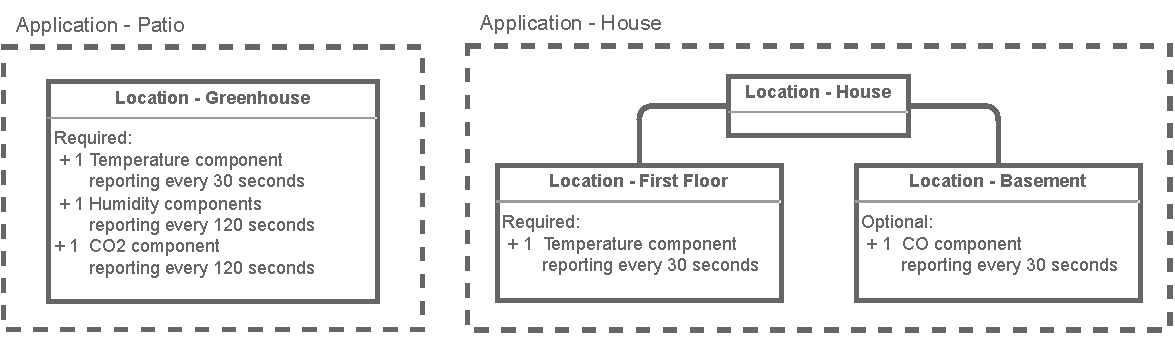
\includegraphics[width=\linewidth]{images/ScenarioB.pdf}
    \vspace{-4mm}
\end{figure}

Para esta simulación, todos los componentes de la aplicación ya estarán ejecutándose, con el problema de que no todos estarán dentro de los parámetros establecidos. Esto requerirá que la aplicación identifique el servicio correspondiente, y realice la reconfiguración de sus parámetros.

De la misma manera que se realizó en escenario experimental A, se realizó la declaración de los estados de referencia de cada una de las aplicaciones, al igual que las directivas para su ejecución. Los YAML de esta declaración, y las directivas definidas, se encuentran en los apéndices \ref{ape:ExpB1}, \ref{ape:ExpB2}, \ref{ape:directivesB1} y \ref{ape:directivesB2}.

Partiendo de todo lo anterior, se definió la serie de pasos a realizar para este primer escenario experimental:

\begin{enumerate}[itemsep=0mm]
    \item Desplegar los servicios de Smart Campus UIS
    \item Desplegar los servicios \textit{Bran} y \textit{DoThing}.
    \item Usando \textit{Lexical}, establecer el estado de referencia de la aplicación Patio y House. 
    \item Declarar en los endpoints de \textit{Bran}, las directivas definidas.
    \item Desplegar los servicios de simulación de datos \textit{Mocker} respecto a las expectativas, tal que el estado sea coherente.
    \item Desplegar los servicios \textit{Looker} para cada una de las aplicaciones.
    \item Matar los servicios desplegados y eliminar uno de los contenedores creados.
    \item Esperar a ejecución de las órdenes \textit{Restart} y \textit{Addition}.
\end{enumerate}